\documentclass[border=6pt]{standalone}
\usepackage{tikz}
\usetikzlibrary{arrows.meta,positioning,calc}
\begin{document}
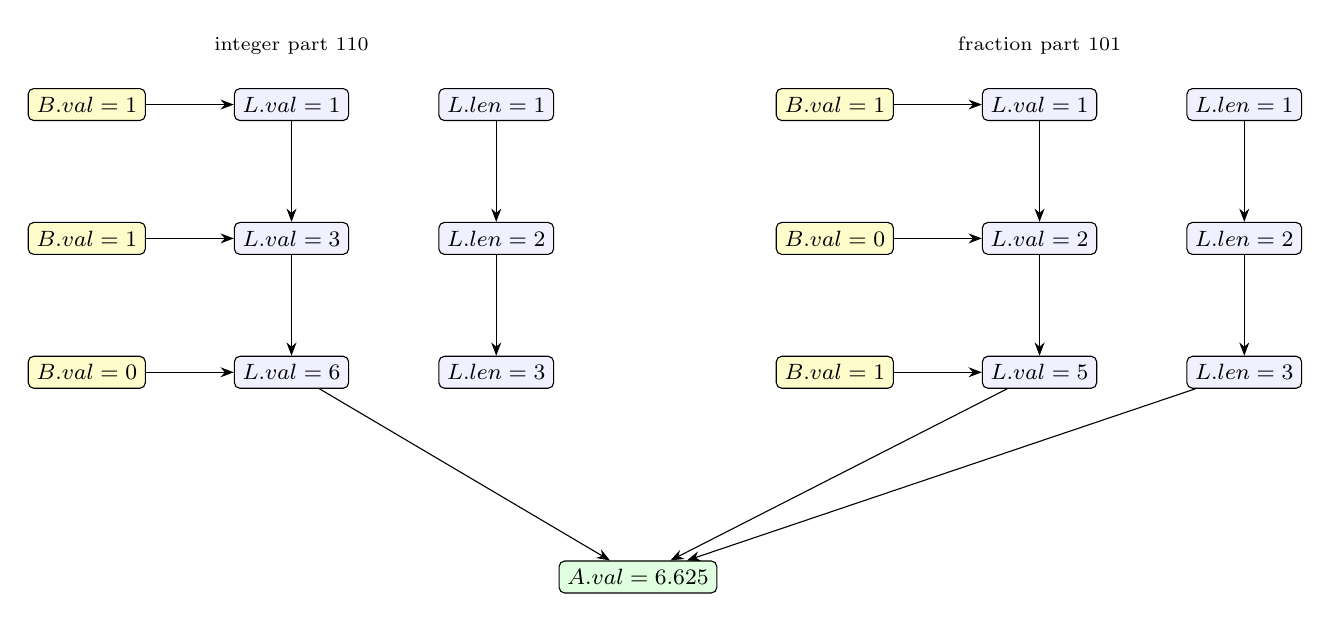
\begin{tikzpicture}[>=Stealth,font=\footnotesize,
 b/.style={draw,rounded corners=2pt,fill=yellow!20,inner sep=3pt},
 a/.style={draw,rounded corners=2pt,fill=blue!6,inner sep=3pt}]
\node[b] (lB1) at (0.00,0.00) {$B.val=1$};
\node[a] (lV1) at (2.60,0.00) {$L.val=1$};
\node[a] (lN1) at (5.20,0.00) {$L.len=1$};
\node[b] (lB2) at (0.00,-1.70) {$B.val=1$};
\node[a] (lV2) at (2.60,-1.70) {$L.val=3$};
\node[a] (lN2) at (5.20,-1.70) {$L.len=2$};
\node[b] (lB3) at (0.00,-3.40) {$B.val=0$};
\node[a] (lV3) at (2.60,-3.40) {$L.val=6$};
\node[a] (lN3) at (5.20,-3.40) {$L.len=3$};
\node[b] (rB1) at (9.50,0.00) {$B.val=1$};
\node[a] (rV1) at (12.10,0.00) {$L.val=1$};
\node[a] (rN1) at (14.70,0.00) {$L.len=1$};
\node[b] (rB2) at (9.50,-1.70) {$B.val=0$};
\node[a] (rV2) at (12.10,-1.70) {$L.val=2$};
\node[a] (rN2) at (14.70,-1.70) {$L.len=2$};
\node[b] (rB3) at (9.50,-3.40) {$B.val=1$};
\node[a] (rV3) at (12.10,-3.40) {$L.val=5$};
\node[a] (rN3) at (14.70,-3.40) {$L.len=3$};
\node[a,fill=green!12] (A) at (7.0,-6.0) {$A.val=6.625$};
\draw[->] (lB1) -- (lV1);
\draw[->] (lB2) -- (lV2);
\draw[->] (lV1) -- (lV2);
\draw[->] (lN1) -- (lN2);
\draw[->] (lB3) -- (lV3);
\draw[->] (lV2) -- (lV3);
\draw[->] (lN2) -- (lN3);
\draw[->] (rB1) -- (rV1);
\draw[->] (rB2) -- (rV2);
\draw[->] (rV1) -- (rV2);
\draw[->] (rN1) -- (rN2);
\draw[->] (rB3) -- (rV3);
\draw[->] (rV2) -- (rV3);
\draw[->] (rN2) -- (rN3);
\draw[->] (lV3) -- (A);
\draw[->] (rV3) -- (A);
\draw[->] (rN3) -- (A);
\node[font=\scriptsize] at (2.6,0.75) {integer part 110};
\node[font=\scriptsize] at (12.1,0.75) {fraction part 101};
\end{tikzpicture}
\end{document}
